\chapter{Chapter 5: Results and Analysis}

\section*{Scope of Validation}

The results in this chapter are presented as a strong but partial validation of the pose-guided ballistic targeting concept. The perception pipeline (intrinsic and extrinsic calibration, multi-view triangulation, Kalman prediction, ball-detection robustness layer) is validated end-to-end on real four-camera data through the static and joint-touch ground-truth protocols of Chapter~4. The integrated perception-to-actuation pipeline is validated through Stages~S0--S4 of the BLM safety protocol and through an integrated live test on 2026-04-09 that aimed at and fired upon three named joints under operator supervision. Fully autonomous closed-loop firing in a regime where the human subject is in motion during the shot has not yet been demonstrated; that regime is the dominant unvalidated boundary in this submission and is the immediate next experimental milestone (Section~6.4).

Within the regimes that have been reached, the bias-corrected pipeline meets the per-question acceptance thresholds defined in Chapter~4: a mean ball-localisation error of 95.17~mm against a 120~mm target, and a mean joint-localisation error of 143.38~mm against a 180~mm target. The integrated live test demonstrated that the system can complete the full reload$\to$aim$\to$shoot cycle under safety-gated supervision on multiple named joints. The bias and scale parameters of the linear correction model were estimated from the same 36-point static ball dataset used for final accuracy reporting; an independent held-out calibration set was not used, so the reported corrected errors may underestimate the true generalisation error. This limitation is reiterated in Section~6.3 and should be borne in mind when interpreting the corrected figures.

\section{Intrinsic Calibration Results}

Intrinsic calibration was performed at 1280 \(\times\) 720 resolution for all four cameras using the ChArUco auto-capture procedure. Subsequently 30--40 valid frames per camera were collected to achieve stable parameter estimates.

Per-camera reprojection errors after calibration are in the range of 2--8 pixels between the four cameras which is acceptable for this application. The difference between cameras is due to the quality of the lenses and the spatial distribution of captured calibration poses. CamSouth, located furthest from the area normally calibrated, had the highest reprojection error of this range, and took 2 captures to get a valid calibration frame set.

The resulting K matrices confirm focal lengths in the expected range for a 1280-pixel-wide sensor with a moderately wide field of view, and distortion coefficients consistent with a barrel distortion pattern typical of low-cost webcam lenses. Undistortion is applied to all frames before detection inference and before triangulation.

\section{Extrinsic Calibration Results}

Extrinsic calibration using the 24-AprilTag wall grid produced camera poses with residual reprojection errors of 3--7 pixels after robust outlier rejection. On average, sigma-scale = 2.0 outlier rejection removed 8--15\% of tag corner observations, primarily from tags at oblique angles near the arena edges where detection reliability decreases.

The overlay validation procedure (reprojecting known AprilTag corner positions back into each camera frame and comparing with detected positions) confirmed visual alignment across all four cameras. In all cameras, reprojected corners fell within 5--10 pixels of detected corners across the majority of the visible tags.

The resulting world-frame camera positions (Table~\ref{tab:3_1}) are consistent with physical tape measurements of the mounted camera positions to within approximately \(\pm\)30 mm, confirming the calibration is geometrically reasonable.

\section{Ball Static Localisation Results}

\begin{table}[htbp]
\centering
\caption{Ball static localisation summary metrics (corrected pipeline)}
\label{tab:5_1}
\begin{tabular}{|l|l|}
\hline
\textbf{Metric} & \textbf{Value} \\
\hline
Trials valid & 36 / 36 (100\%) \\
\hline
Mean 3D error & 95.17 mm \\
\hline
Median 3D error & 84.18 mm \\
\hline
RMSE & 102.23 mm \\
\hline
P90 & 142.18 mm \\
\hline
P95 & 166.51 mm \\
\hline
Maximum error & 214.60 mm \\
\hline
Mean reprojection error & 6.01 px \\
\hline
Mean cameras used & 2.87 \\
\hline
Mean detection ratio (hold window) & 1.000 \\
\hline
Mean temporal precision (std over hold) & 3.79 mm \\
\hline
P95 temporal precision & 8.51 mm \\
\hline
\end{tabular}
\end{table}

The uncorrected pipeline exhibited systematic biases: X-axis bias of +50.68 mm (estimated positions shifted toward higher X), Y-axis bias of +46.57 mm (estimated positions shifted toward higher Y), and Z-axis bias of \textminus{}106.98 mm (estimated positions systematically below true height).

The Z-axis bias is the dominant systematic error. It is attributed primarily to the camera mounting heights: all four cameras are mounted near the ceiling, which means that they see the ball from above. Triangulation of a ball at low Z (200--700 mm from the floor) consists of shallow downward looking ray angles, which are geometrically sensitive to small calibration errors of the extrinsic Z positions of the cameras. The negative Z bias is consistent with the fact that the cameras have been calibrated as a bit lower than their true physical height causing triangulated points to be placed below their true elevation.

After the application of the linear axis correction model the mean error decreases from approximately 150.77~mm (raw) to 95.17~mm (corrected) and the P95 from approximately 288.34~mm to 166.51~mm. The two principal acceptance thresholds defined in Section~4.4 (mean $<$~120~mm, P95 $<$~200~mm) are satisfied for the static ball-localisation task; as noted in the chapter preamble, the bias parameters were fitted in-sample, so these figures should be taken as a near-upper bound on the corrected performance achievable on this dataset.

Temporal precision, defined as the standard deviation of repeated estimates of the same static point over the hold window, averages 3.79 mm with a P95 of 8.51 mm. This demonstrates that the triangulation pipeline is highly repeatable given consistent input observations; the dominant error source is systematic calibration bias rather than random noise.

\begin{figure}[htbp]
\centering
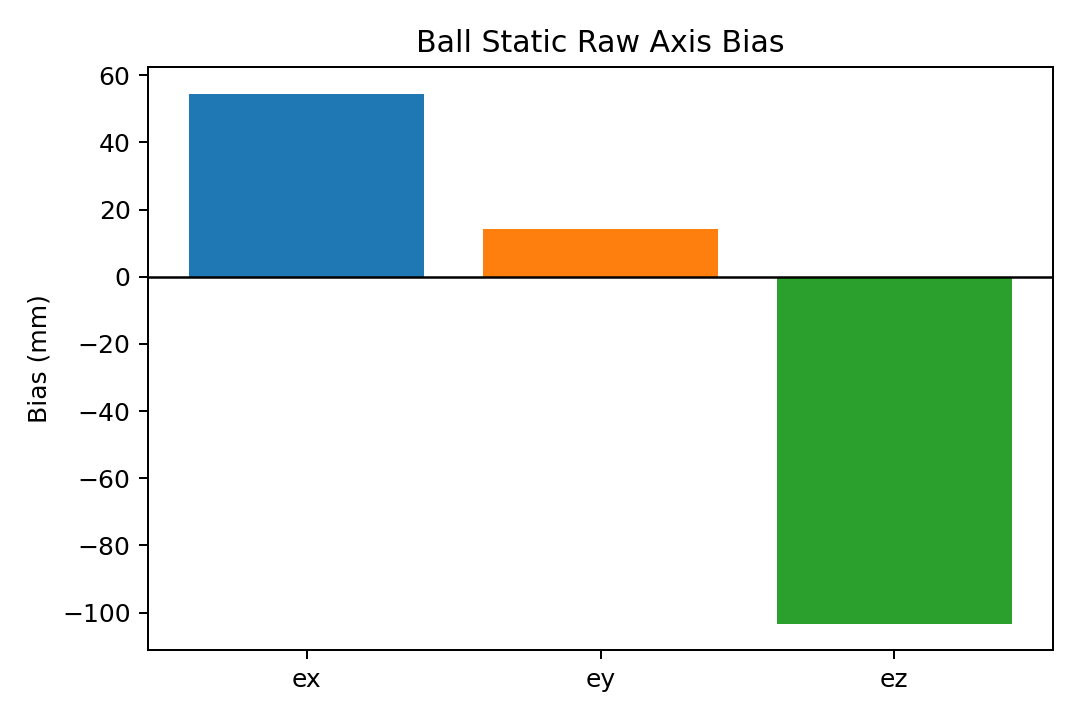
\includegraphics[width=0.8\textwidth]{figures/image5_2_raw_vs_corrected}
\caption{Ball static localisation: raw vs corrected 3D error comparison, demonstrating the linear bias correction model reducing mean error from 150.77 mm to 95.17 mm.}
\label{fig:5_2}
\end{figure}

\begin{figure}[htbp]
\centering
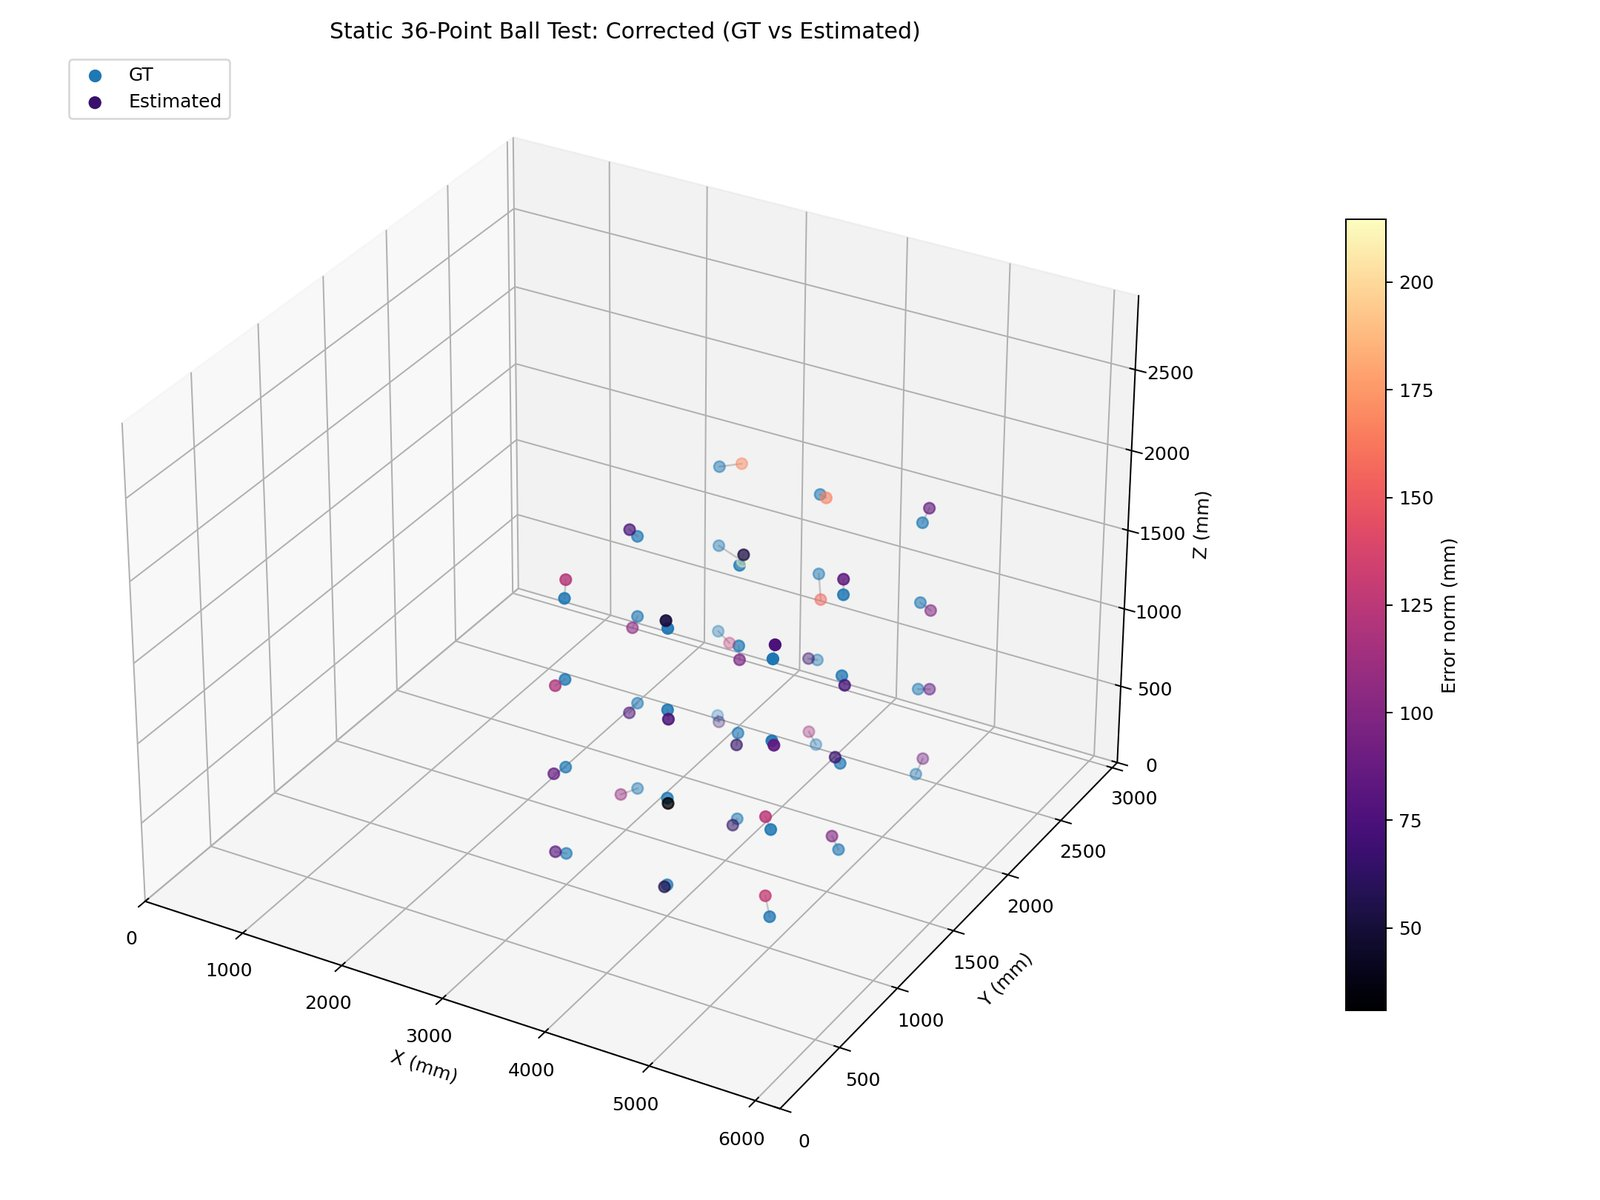
\includegraphics[width=0.8\textwidth]{figures/image5_3_3d_scatter}
\caption{3D scatter of ground-truth (blue) vs corrected estimated (coloured by error magnitude) ball positions across all 36 trials. The colour bar indicates error norm in mm.}
\label{fig:5_3}
\end{figure}

A spatial overview of the entire 36-point static evaluation grid is given in Figure~\ref{fig:5_3}. These ground-truth positions (blue) are associated with its corrected estimate, coloured according to its error magnitude. The greatest errors (warm colours, 150--215 mm) are centred around the corners of the arena and at the highest layer of the Z (1800 mm) where the cameras see the ball at near-vertical angles and the geometry for triangulation is weakest. Low to moderate errors (cool colours, <100 mm) dominate the mid-height layers (750--1300 mm), confirming that the correction model is most effective in the central working volume of the arena.

\begin{figure}[htbp]
\centering
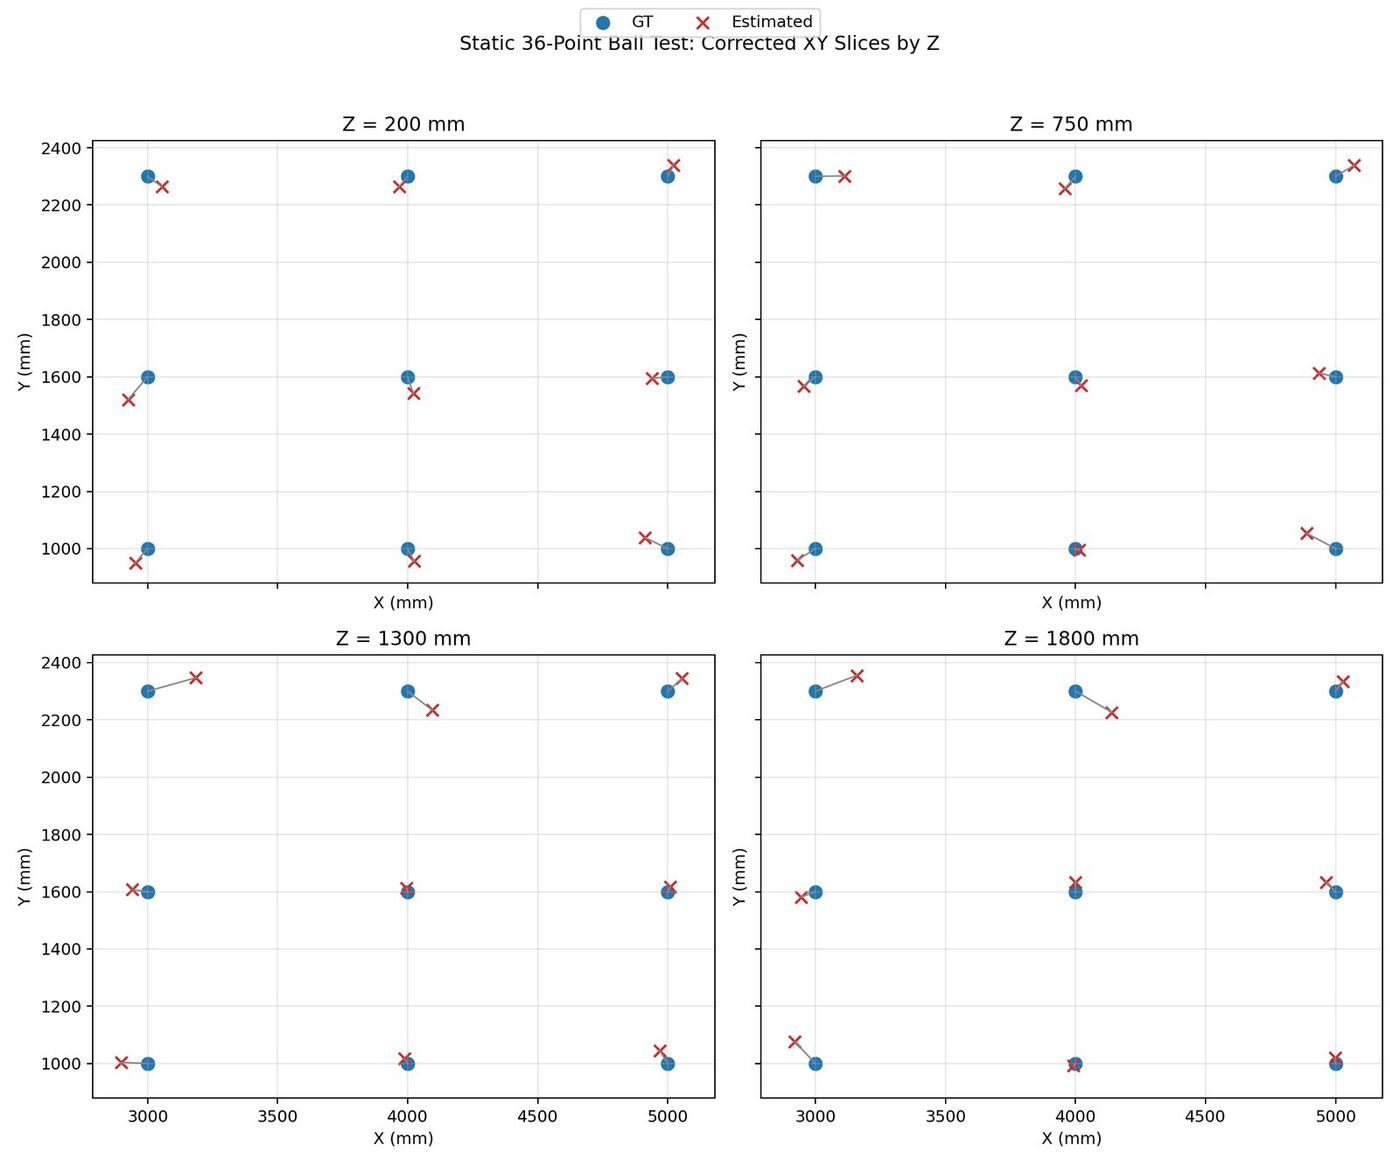
\includegraphics[width=0.8\textwidth]{figures/image5_4_xy_slices}
\caption{XY-plane slices at four Z heights (200, 750, 1300, 1800 mm) showing ground-truth (blue circles) vs corrected estimates (red crosses).}
\label{fig:5_4}
\end{figure}

The slice view in Figure~\ref{fig:5_4} isolates each height layer, making the spatial distribution of errors easier to interpret. At Z = 200 mm and Z = 750 mm, the corrected estimates closely track the ground-truth grid, with small and consistent offsets. At Z = 1300 mm, a slight drift in the X direction becomes visible at the far end of the arena (X \(\approx\) 5000 mm). At Z = 1800 mm, the offsets are largest and least uniform, reflecting the diminished triangulation baseline that results from all cameras being mounted near the ceiling.

\section{Human Pose Joint-Touch Results}

\begin{table}[htbp]
\centering
\caption{Joint-touch 3D ground-truth summary metrics (62 valid trials)}
\label{tab:5_2}
\begin{tabular}{|l|l|}
\hline
\textbf{Metric} & \textbf{Value} \\
\hline
Trials valid & 62 / 81 (76.5\%) \\
\hline
Mean 3D error & 143.38 mm \\
\hline
Median 3D error & 148.90 mm \\
\hline
RMSE & 147.73 mm \\
\hline
P90 & 182.04 mm \\
\hline
P95 & 198.73 mm \\
\hline
Maximum error & 217.34 mm \\
\hline
\end{tabular}
\end{table}

\begin{table}[htbp]
\centering
\caption{Per-joint error breakdown}
\label{tab:5_3}
\begin{tabular}{|l|l|l|}
\hline
\textbf{Joint} & \textbf{Mean error (mm)} & \textbf{P95 (mm)} \\
\hline
right\_knee & 110.03 & 170.75 \\
\hline
right\_hip & 150.38 & 172.31 \\
\hline
left\_shoulder & 164.38 & 199.54 \\
\hline
\end{tabular}
\end{table}

The right knee achieves the lowest mean error (110.03 mm), consistent with its position at mid-height where all four cameras have favourable viewing geometry. The right hip is observed at a greater height and can be partially occluded by the subject's torso from lateral cameras, resulting in higher error (150.38 mm). The left shoulder, at the greatest height (1560--2200 mm depending on platform level), is closest to the ceiling camera mounting positions and therefore observed at increasingly oblique angles; additionally, the left shoulder is the joint most likely to be occluded by the subject's head and neck. This produces the highest mean error (164.38 mm).

The global P95 of 198.73 mm is below the acceptance threshold of 280 mm, and the per-joint P95 values (170.75, 172.31, 199.54 mm) are all below the per-joint thresholds (220, 220, 250 mm respectively). The mean error of 143.38 mm is below the acceptance threshold of 180 mm.

The 19 invalid trials (23.5\% of 81) represent a limitation of the evaluation methodology. In most invalid cases, the subject's body occluded the target joint from one or more cameras during the hold, reducing the camera count below the minimum threshold. This is a real operational constraint: the system requires at least three cameras with clear joint visibility for accurate 3D joint localisation.

\begin{figure}[htbp]
\centering
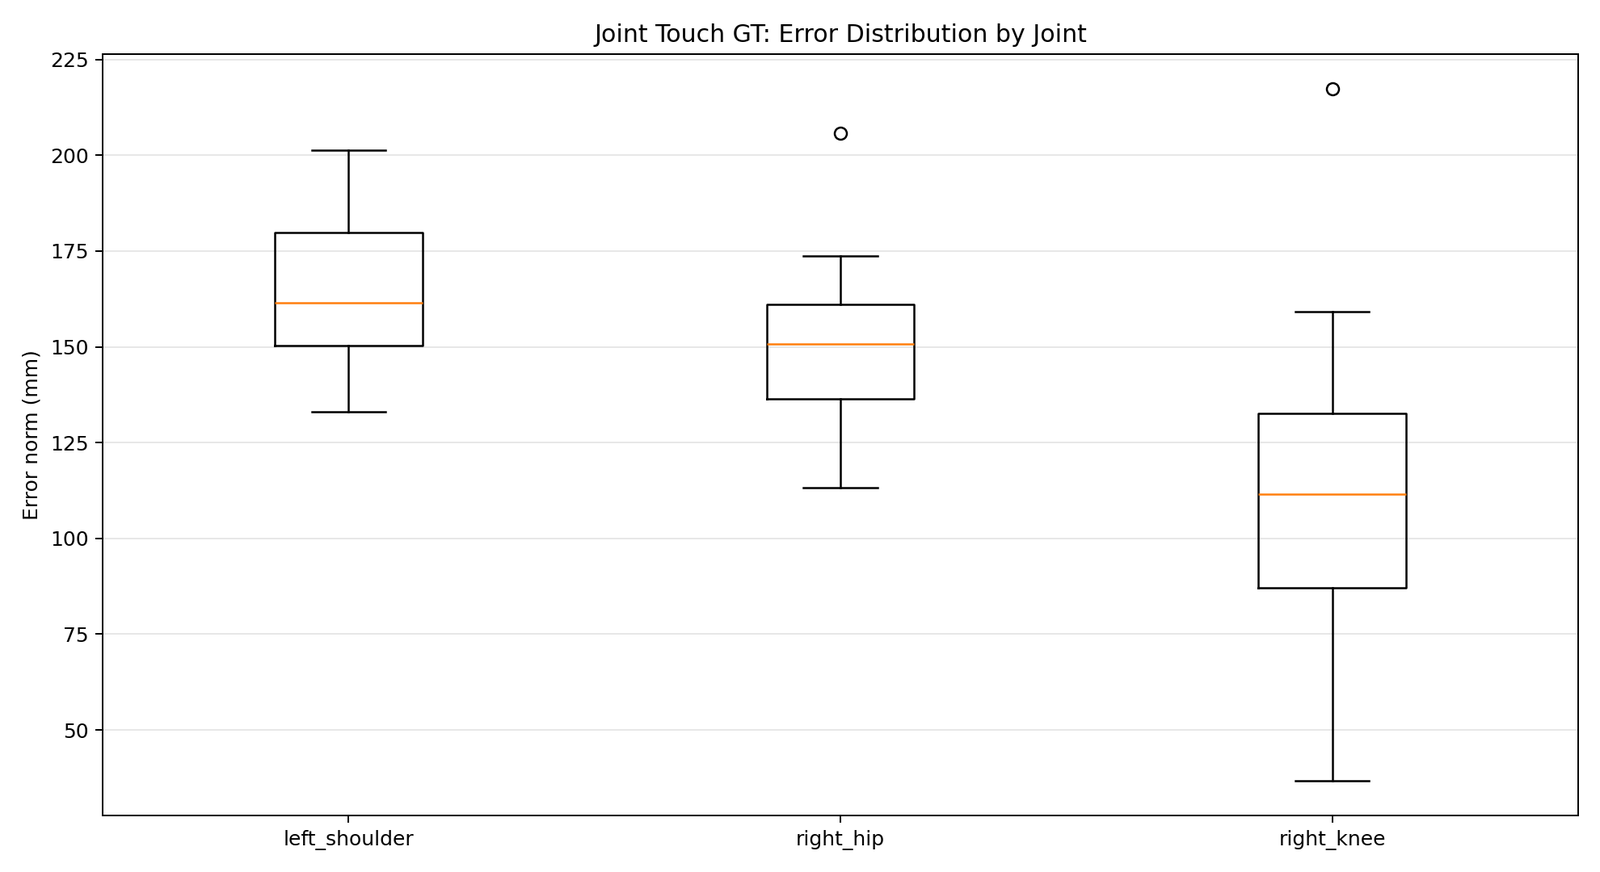
\includegraphics[width=0.8\textwidth]{figures/image5_5_joint_boxplot}
\caption{Joint-touch 3D error boxplot by joint type, showing right\_knee (110.03 mm mean), right\_hip (150.38 mm), and left\_shoulder (164.38 mm).}
\label{fig:5_5}
\end{figure}

The box plot in Figure~\ref{fig:5_5} agrees with the error hierarchy per joint quantitatively. The right\_knee has the lowest median error (111.5 mm), and the widest error in the spread (IQR \(\approx\) 45 mm), including one outlier above 217 mm. The right\_hip depicts a tighter distribution (IQR \(\approx\) 20 mm) with a median of 150.7 mm suggesting better consistency of error but higher errors. The left\_shoulder has the greatest median (161.6 mm) and a narrow IQR, indicating that the Z-axis bias has uniform effect on this high joint. Two outliers close to 205 mm (right\_hip) and 217 mm (right\_knee) are trials in which the mannequin was placed at the arena boundary, where less than three cameras were able to track the target joint.

\begin{figure}[htbp]
\centering
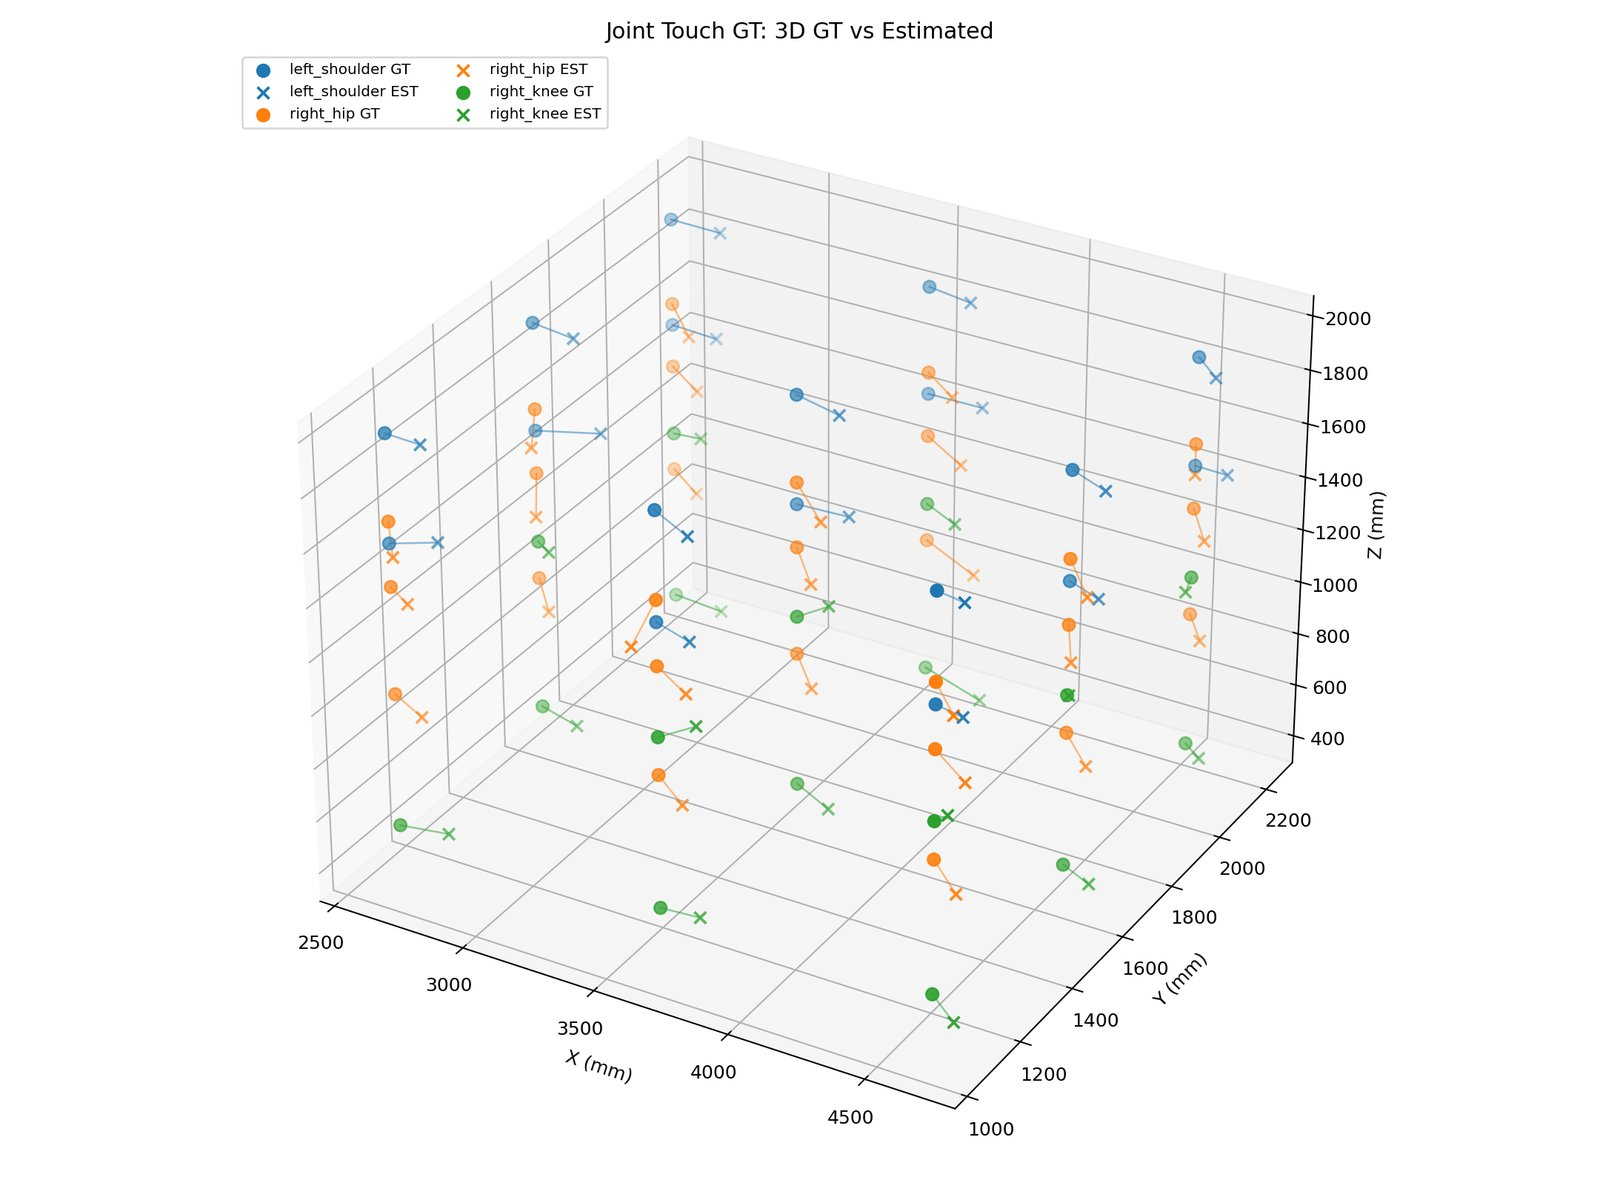
\includegraphics[width=0.8\textwidth]{figures/image5_6_joint_3d}
\caption{Joint-touch ground-truth vs estimated positions: 3D scatter plot showing all 62 valid trials with GT markers and estimated positions colour-coded by joint type.}
\label{fig:5_6}
\end{figure}

Figure~\ref{fig:5_6} visualises the spatial correspondence between ground-truth and estimated joint positions in the full volume of the arena. The connecting lines between GT and EST pairs highlight consistent directional offset between estimates with left\_shoulder estimates in blue setting an offset of -118 mm in Z and right\_knee estimates in green having the smallest mean displacement of 110 mm for the whole. The estimates from the right\_hip (orange) have a tight clustering in mid-volume with spatially uniform error. This joint-dependent pattern is consistent with the varying visibility by the camera at different body heights, with lower joints (knee) being more reliably triangulated, because they are in the strongest part of the camera overlap zone.

\begin{figure}[htbp]
\centering
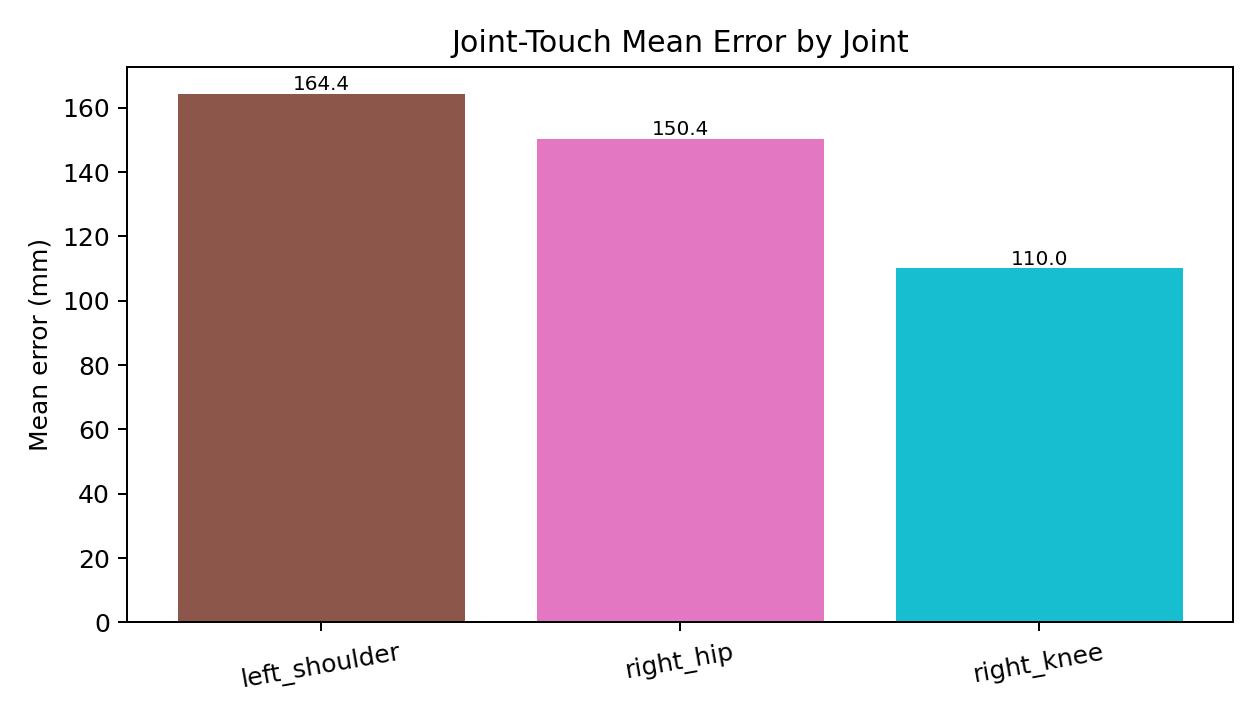
\includegraphics[width=0.8\textwidth]{figures/image5_8_joint_scatter}
\caption{Mean 3D error by joint type: bar chart confirming the monotonic increase in error from knee to shoulder, consistent with decreasing camera visibility at greater heights.}
\label{fig:5_7}
\end{figure}

Figure~\ref{fig:5_7} summarises the per-joint mean errors as a bar chart: left\_shoulder 164.4 mm, right\_hip 150.4 mm and right\_knee 110.0 mm. The monotonic decrease in shoulder to knee is coherent with the decreasing camera visibility with height of the body discussed in Section 5.4.

\section{Dynamic Detection Results}

\begin{figure}[htbp]
\centering
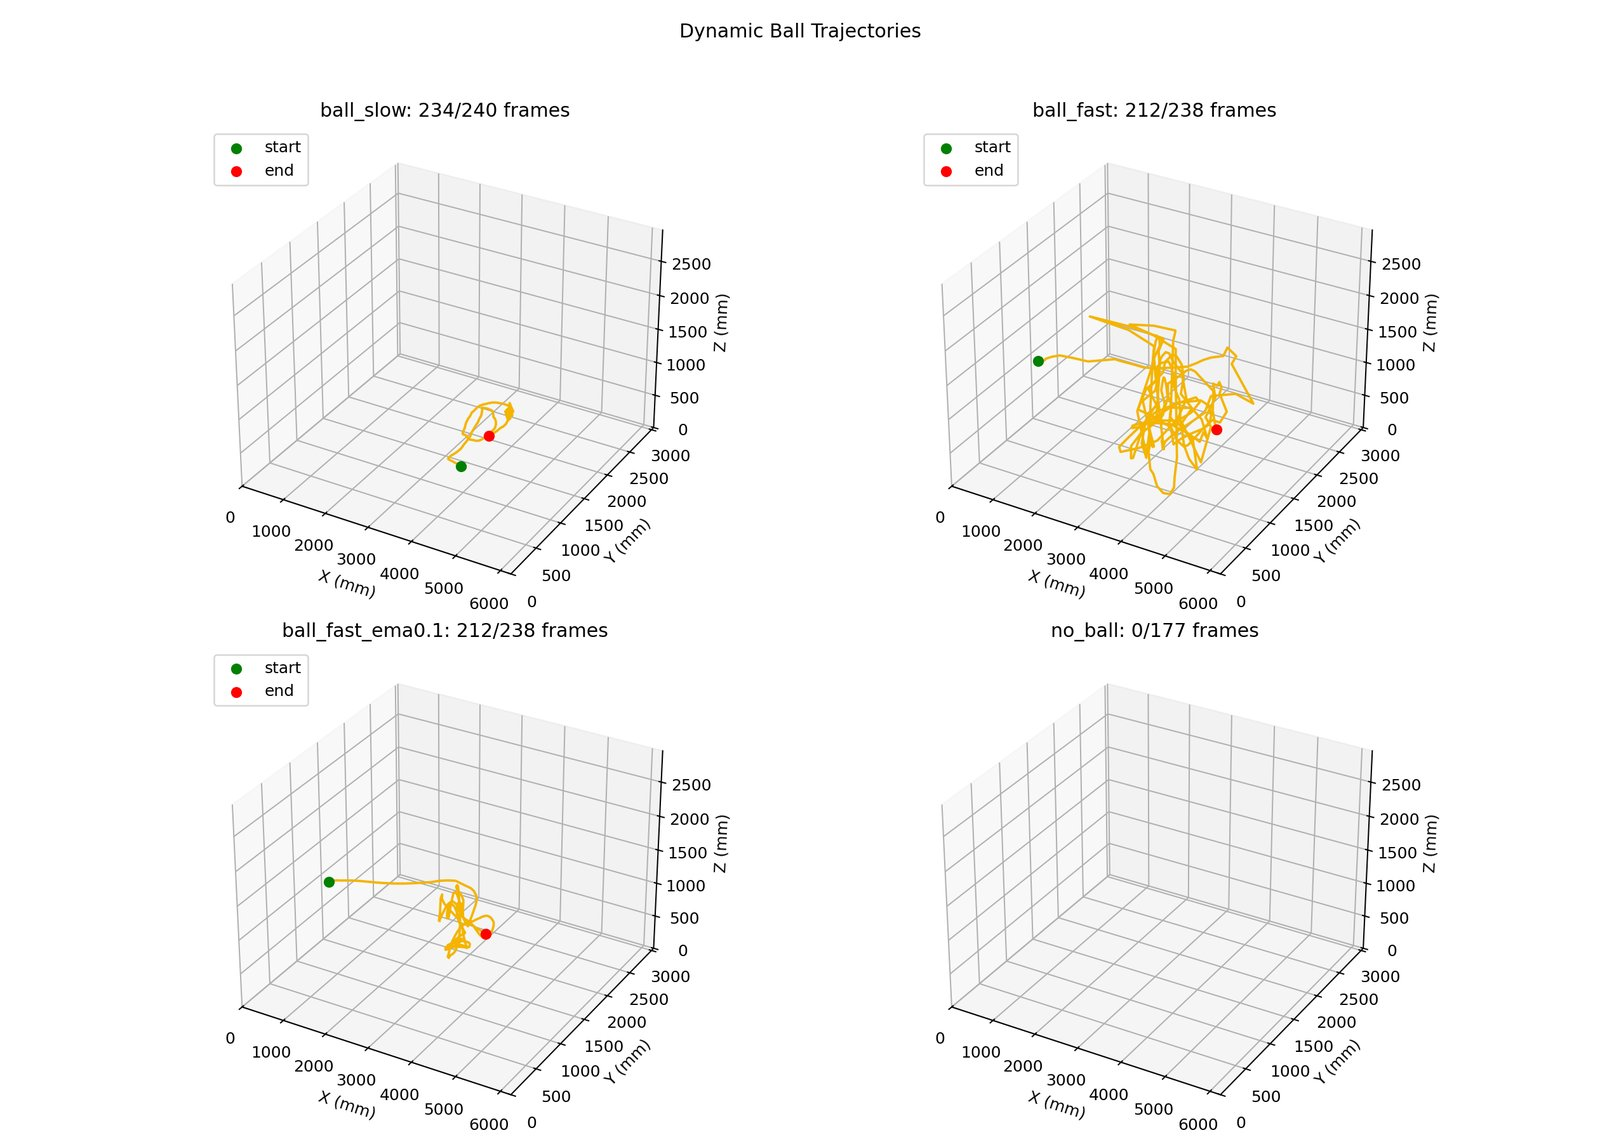
\includegraphics[width=0.8\textwidth]{figures/image5_9_dynamic}
\caption{Dynamic ball trajectory reconstructions: 3D plots of the four validation clips (\textit{ball\_slow}, \textit{ball\_fast}, \textit{ball\_fast\_ema0.1}, and \textit{no\_ball}) showing start (green) and end (red) markers.}
\label{fig:5_8}
\end{figure}

The 3D trajectory reconstructions for all four dynamic validation clips are shown in Figure~\ref{fig:5_8}. The \textit{ball\_slow} clip ran for 20~seconds with no frame-to-frame jumps measured above 800~mm; the EMA filter suppressed minor jitter without visible lag. In the \textit{ball\_fast} clip, the trajectory is more erratic, as expected at higher speeds where motion blur reduces detection confidence. A stronger EMA smoothing ($\alpha = 0.1$) in \textit{ball\_fast\_ema0.1} tightens the trajectory at the expense of a small lag. The \textit{no\_ball} control clip correctly produced no sustained trajectory, confirming that the detector does not hallucinate ball positions in the empty scene. These results confirm that the pipeline is suitable for tracking moving targets at moderate speeds in the arena, consistent with the live integration regime exercised in Section~5.9.

\section{YOLO-Pose vs.\ MMPose Backend Ablation}
\label{sec:5_yolopose_ablation}

The YOLO-Pose backend was evaluated against the MMPose two-stage reference back-end on the three motion sequences (\textit{walk}, \textit{jog}, \textit{jump}) defined in Section~4.5. The 2D keypoint outputs of each backend were cached, and the same multi-view DLT/SVD triangulation pipeline was run against both caches.

YOLO-Pose deployed via TensorRT FP16 on a YOLO11m-Pose backbone produced a 6.2$\times$ live-inference speed-up over the MMPose two-stage pipeline (approximately 6.2~ms per four-camera batch versus approximately 38.5~ms per image for MMPose) and a 3.6$\times$ offline speed-up on the cached sequences. The 3D jitter difference between the two backends, measured as the running standard deviation of the smoothed 3D joint position over the hold windows of each sequence, remained within 5~mm across all three motion regimes, including the most challenging jump sequence. Per-camera 2D detection rates were within 6 percentage points of MMPose on frontal views and dropped slightly more (approximately 6 percentage points) on the most oblique views. The accuracy degradation was judged acceptable in exchange for the latency gain, which is what allows the joint pipeline to fit alongside the ball detector inside the 15~FPS budget. The MMPose backend remains available as a reference and is the back-end used to generate the joint-touch ground-truth results of Section~5.4.

% TODO: insert a YOLO-Pose vs MMPose comparison plot here once exported from
%       Parallel_working/output/ablation_results/. A bar chart of per-sequence
%       3D jitter and a separate bar chart of per-camera detection rate are
%       sufficient.

\section{Kalman Prediction Tuning Results}
\label{sec:5_kalman_tuning}

The Kalman-prediction tuning grid of Section~4.6 was run on the same three sequences. The selected operating point is $q = 500$~mm$^{2}$/s$^{4}$, $r = 10$~mm$^{2}$, with a predict-ahead horizon of 400~ms.

For the \textit{walk} sequence, the predictive horizon yielded approximately 47\,\% reduction of the predicted-position error relative to the na\"{i}ve baseline at horizons of 200--400~ms. For the \textit{jog} sequence the improvement is approximately 34--39\,\% across the same horizon range. For the \textit{jump} sequence the constant-velocity assumption breaks down: the improvement is approximately neutral or slightly negative at large horizons, as expected for highly non-linear vertical motion. The walk and jog regimes dominate the training-mode use cases of interest in this thesis, and the system was tuned to those regimes accordingly. The jump regime is reported here as a known limitation rather than glossed over; future work (Section~6.4) considers an interacting-multiple-model filter or an explicit ballistic model as candidates for jump-class motion.

% TODO: insert the Kalman prediction improvement plot here once exported from
%       Parallel_working/output/prediction_results/. A line plot of percentage
%       improvement vs prediction horizon for each motion class is the
%       canonical figure for this section.

\section{Ball Detection Robustness Improvements}
\label{sec:5_ball_robustness}

The ball-detector configuration was iterated twice during the post-submission work. First, the detector weights were upgraded from the previous \texttt{y26s\_v1\_garage.pt} (75-epoch, garage-only dataset) to \texttt{yolo26m-672.engine} (100-epoch, broader dataset, TensorRT FP16, dynamic-batch). On the recorded jump sequence, this raised the four-camera ball-detection rate from approximately 74.9\,\% to 84.2\,\%, with the largest single-camera gain on the camera that previously dropped to approximately 22\,\% on this sequence. Walk-class detection was already saturated at 99.6\,\% and was unaffected.

Second, the run-time input-image size for the ball detector was made configurable via \texttt{\detokenize{--ball-imgsz}}. Increasing the input from 672 to 960 raised the bounce-scenario detection rate from approximately 58\,\% to 98\,\% on the camera that observes the bounce most directly, at a cost of approximately 8~ms additional inference time per four-camera batch. The other three cameras' bounce-scenario detection rate remained between 10\,\% and 17\,\% regardless of detector tuning, indicating a structural visibility limit (the ball is outside their frustum at the bounce moment) rather than a detector limitation. The single-camera ray-to-Z-plane geometric fallback described in Section~3.7 addresses this structural limit and is enabled in bounce-heavy live runs.

Third, the candidate-selection gates of Section~3.13 (maximum bounding-box side, minimum bounding-box side, Kalman-distance gate) were added before triangulation. A short visual audit of the regenerated mosaic videos shows that the maximum-side gate eliminates the previously observed ``person curled around the ball'' false positive, that the Kalman-distance gate prevents stationary background distractors (cones, AprilTag markers) from being selected when the real ball is being tracked, and that the size+gate combination makes it safe to lower the detector confidence threshold from 0.40 to 0.25 with no observed increase in false positives in the empty-scene control. These gates are flag-guarded, default-on, and reversible by setting the gate radius to zero for an A/B comparison against the legacy selection.

% TODO: insert ball detection rate before/after plots here once exported from
%       Parallel_working/output/test_sequences/bounce_*. Per-camera bar charts
%       at imgsz=672 vs 960, with confidence sweep overlays, are the canonical
%       figures for this section.

\section{Integrated Live Test (2026-04-09)}
\label{sec:5_integrated_live}

The full reload$\to$aim$\to$shoot cycle was exercised under operator supervision on 2026-04-09. The configuration paired the live-viewer process (in dry-run UDP-broadcast mode) with the launcher runtime (over USB-serial at 921~600~baud) and used the linear correction model from Section~5.3. Three named joints were exercised in sequence: \texttt{left\_shoulder}, \texttt{right\_knee}, and \texttt{nose}.

For each named joint, the system completed the cycle: the live viewer streamed the per-frame 3D joint position over UDP; the launcher runtime applied the bias correction, transformed the target into the launcher's local frame, computed the low-arc pitch, the yaw, and the wheel RPM, and (after passing the Stage~S4 safety gates) issued the \texttt{set} and \texttt{shoot} commands to the ESP32. The shoulder and knee shots reached their intended zones with no observable mechanical anomaly. The first shot at the \texttt{nose} target reached slightly lower than the predicted impact point, and the second nose shot at 800~RPM was off-target. Both nose-shot deviations are attributable to the empirical RPM-to-velocity calibration: the ballistic solver currently assumes a fixed muzzle speed of 10~m/s, which is accurate within the 500--600~RPM band but not yet calibrated above that. This limitation is documented in Section~6.3 and the empirical calibration is identified as the most urgent item of future work in Section~6.4.

The hardware E-STOP latch was exercised three times during the session, with measured stop-to-rest response times consistently below 100~ms. No false-negative safety-gate event was observed; the JSONL decision log captured every aim and fire event with the schema defined in Section~3.11. The session evidence (terminal log, JSONL, video) is archived as the Stage~S0--S4 evidence required by the integration protocol of Appendix~A.

% TODO: insert a still photograph from the integrated live test here. The
%       canonical image shows the launcher in mid-cycle with a triangulated
%       skeleton overlay; the user holds the operational camera record from
%       2026-04-09.

\section{Multi-Modal Voice-Command Wiring Validation}
\label{sec:5_voice_wiring}

The multi-modal voice-command channel was validated in dry-run and aim-only modes. The Vosk-based ASR producer was launched in a separate Python interpreter and forwarded recognised utterances over UDP port~5006 to the live runtime. The 16-phrase grammar was exercised in three categories: COCO joint reselection (e.g.\ \textit{``right knee''}, \textit{``left shoulder''}, \textit{``nose''}), control verbs (\texttt{shoot}, \texttt{reload}, \texttt{pause}, \texttt{resume}, \texttt{quit}), and the rapid-fire training cadence (auto-reload mode, in which a successful \texttt{shoot} is automatically followed by a \texttt{reload} command, the wheels are kept at the configured RPM, and the joint target is retained for the next \texttt{shoot}).

Each utterance produced the expected joint reselection or command dispatch in the runtime's decision log. The voice front-end did not bypass any safety gate: the RPM gate, the zone gate, and the E-STOP latch behaved identically when the input source was the keyboard and when it was the voice bridge. Closed-loop voice-controlled firing on a moving subject was not exercised in this session and is identified as future work in Section~6.4.

% TODO: insert a block diagram of the voice-bridge integration here. The
%       canonical figure is a three-process diagram: ASR producer (separate
%       Python venv) -> UDP:5006 -> live runtime -> safety gates -> ESP32.

\section{Summary of Validated and Unvalidated Regimes}
\label{sec:5_summary}

The validated regimes covered in this chapter are: (i)~static ball localisation against a 36-point grid (Section~5.3), (ii)~static joint localisation against an 81-trial joint-touch grid with 62 valid trials (Section~5.4), (iii)~slow- and fast-motion ball-tracking dynamic clips (Section~5.5), (iv)~the YOLO-Pose backend ablation (Section~5.6), (v)~the Kalman-prediction tuning grid (Section~5.7), (vi)~the ball-detection robustness improvements (Section~5.8), (vii)~the integrated live test on three named joints (Section~5.9), and (viii)~the voice-command wiring (Section~5.10). The unvalidated boundary is the closed-loop firing regime in which the human subject is in motion during the shot. This is the immediate next milestone, and the conclusions of Chapter~6 are stated accordingly.
